%%%%%%%%%%%%%%%%%%%%%%%%%%%%%%%%%%%%%
% Short Sectioned Assignment
% LaTeX Template
% Version 1.0 (5/5/12)
%
% This template has been downloaded from:
% http://www.LaTeXTemplates.com
%
% Original author:
% Frits Wenneker (http://www.howtotex.com)
%
% License:
% CC BY-NC-SA 3.0 (http://creativecommons.org/licenses/by-nc-sa/3.0/)
%
%%%%%%%%%%%%%%%%%%%%%%%%%%%%%%%%%%%%%%%%%

%----------------------------------------------------------------------------------------
%	PACKAGES AND OTHER DOCUMENT CONFIGURATIONS
%----------------------------------------------------------------------------------------

\documentclass[paper=a4, fontsize=11pt]{scrartcl} % A4 paper and 11pt font size
\usepackage{graphicx}
\usepackage{subcaption}
\usepackage[normalem]{ulem}
\useunder{\uline}{\ul}{}
\usepackage{listings}
\usepackage{color} %red, green, blue, yellow, cyan, magenta, black, white
\definecolor{mygreen}{RGB}{28,172,0} % color values Red, Green, Blue
\definecolor{mylilas}{RGB}{170,55,241}

\lstset{language=Matlab,%
    basicstyle=\ttfamily,
    breaklines=true,%
    morekeywords={matlab2tikz},
    keywordstyle=\color{blue},%
    morekeywords=[2]{1}, keywordstyle=[2]{\color{black}},
    identifierstyle=\color{black},%
    stringstyle=\color{mylilas},
    commentstyle=\color{mygreen},%
    showstringspaces=false,%without this there will be a symbol in the places where there is a space
    numbers=left,%
    numberstyle={\tiny \color{black}},% size of the numbers
    numbersep=9pt, % this defines how far the numbers are from the text
    emph=[1]{for,end,break},emphstyle=[1]\color{red}, %some words to emphasise
    %emph=[2]{word1,word2}, emphstyle=[2]{style},    
}

\usepackage{gensymb}
\usepackage{float}
\usepackage{graphicx}
\usepackage{subcaption}
\usepackage[T1]{fontenc} % Use 8-bit encoding that has 256 glyphs
\usepackage{fourier} % Use the Adobe Utopia font for the document - comment this line to return to the LaTeX default
\usepackage[english]{babel} % English language/hyphenation
\usepackage{amsmath,amsfonts,amsthm,mathtools} % Math packages
\usepackage{booktabs}
\usepackage{listings}
\usepackage{color}
\usepackage{lipsum} % Used for inserting dummy 'Lorem ipsum' text into the template

\usepackage{sectsty} % Allows customizing section commands
\allsectionsfont{\centering \normalfont\scshape} % Make all sections centered, the default font and small caps

\usepackage{fancyhdr} % Custom headers and footers
\pagestyle{fancyplain} % Makes all pages in the document conform to the custom headers and footers
\fancyhead{} % No page header - if you want one, create it in the same way as the footers below
\fancyfoot[L]{} % Empty left footer
\fancyfoot[C]{} % Empty center footer
\fancyfoot[R]{\thepage} % Page numbering for right footer
\renewcommand{\headrulewidth}{0pt} % Remove header underlines
\renewcommand{\footrulewidth}{0pt} % Remove footerabout:preferences#search uabout:preferences#searchnderlines
\setlength{\headheight}{13.6pt} % Customize the height of the header

\numberwithin{equation}{section} % Number equations within sections (i.e. 1.1, 1.2, 2.1, 2.2 instead of 1, 2, 3, 4)
\numberwithin{figure}{section} % Number figures within sections (i.e. 1.1, 1.2, 2.1, 2.2 instead of 1, 2, 3, 4)
\numberwithin{table}{section} % Number tables within sections (i.e. 1.1, 1.2, 2.1, 2.2 instead of 1, 2, 3, 4)

\setlength\parindent{0pt} % Removes all indentation from paragraphs - comment this line for an assignment with lots of text

\DeclarePairedDelimiterX{\norm}[1]{\lVert}{\rVert}{#1}

%----------------------------------------------------------------------------------------
%	TITLE SECTION
%----------------------------------------------------------------------------------------

\newcommand{\horrule}[1]{\rule{\linewidth}{#1}} % Create horizontal rule command with 1 argument of height

\title{	
\normalfont \normalsize 
\textsc{Monash University} \\ [25pt] % Your university, school and/or department name(s)
\horrule{0.5pt} \\[0.4cm] % Thin top horizontal rule
\huge MTH3011 - Assignment 02 \\ % The assignment title
\horrule{2pt} \\[0.5cm] % Thick bottom horizontal rule
}

\author{Robert A. Koch} % Your name

\date{\normalsize\today} % Today's date or a custom date

\begin{document}

\maketitle % Print the title
\pagebreak

%----------------------------------------------------------------------------------------
%	PROBLEM 1
%----------------------------------------------------------------------------------------

\section*{Problem 01 - Nondimensionalization}

To solve all the problems in this assignment the function needs to be non-dimensionalized so that the units are removed and the equation becomes more generalised. The original equation in \ref{eq:original} can be non-dimensionalized by using the scaling values defined in \ref{eq:scaling}.

\begin{equation} \label{eq:original}
	\dfrac{\partial P}{\partial t} = -\dfrac{\partial P}{\partial a} - \mu(a)P(a,t)
\end{equation}

In these equations $a,t$ are independant variables, and $P$ is the dependant function. $a_{max}$ and $P_{max}$ are the maximum values of $a$ and $P$ respectivly. 

\begin{equation} \label{eq:scaling}
	\tau = t/a_{max} 
	\qquad 
	x = a/a_{max}
	\qquad
	\phi=P/P_{max}
	\qquad
	\phi(x,\tau) = a_{max}\mu(x\cdot a_{max})
\end{equation}

By rearranging the values in \ref{eq:scaling} alternative values for each of the variables in \ref{eq:original} can be found. 

\begin{equation} \label{eq:scaling2}
	t = a_{max} 
	\qquad 
	a = x\cdot a_{max}
	\qquad
	P=\phi\cdot P_{max}
\end{equation}

The values in \ref{eq:scaling2} can be inserted into \ref{eq:original} to get the non-dimensionalized form, this is shown in \ref{eq:nond}. The since $P_{max}$ and $a_{max}$ are constants they can be removed from the partial derivatives and cancelled out. This leaves the final equation.

\begin{align} 
	\label{eq:nond}
	\dfrac{\partial \phi P_{max}}{\partial a_{max}\tau} = -\dfrac{\partial \phi P_{max}}{\partial x a_{max}} - \mu(x\cdot a_{max})\phi P_{max} \\
	\dfrac{\partial\phi}{\partial\tau}\dfrac{P_{max}}{a_{max}} = -\dfrac{\partial\phi}{\partial x}\dfrac{P_{max}}{a_{max}} - \mu(x\cdot a_{max})\phi P_{max} \\
	\dfrac{\partial\phi}{\partial\tau} = -\dfrac{\partial\phi}{\partial x}-\mu(x\cdot a_{max})\phi a_{max} \\
	\dfrac{\partial\phi}{\partial\tau} + \dfrac{\partial\phi}{\partial x}= -\phi\lambda(x)
\end{align}

Following up, if $\lambda$ is nonzero its maximum value must be 1. The reason for this is quite simple. Because $\lambda(x) = a_{max}\mu(x a_{max})$ it is dependant on the death rate of the population by age, at the maximum age an individual can live to the mortality rate will be 100\%. This is what $\lambda$ represents, and since nobody can be older than the oldest person by definition the equation can't be more than 1.

\section*{Problem 02 - Solving}
My approach to all the problems in this assignment is to solve the general equation first before simplifying it.

\begin{equation} \label{eq:toSolve}
		\dfrac{\partial\phi}{\partial\tau} + \dfrac{\partial\phi}{\partial x}= -\phi\lambda(x)
\end{equation}

The equation in \ref{eq:toSolve} can be solved using the method of characteristics. The first step is to identify the characteristic curves along which this equation will be solved. This is done by first identifying that the change in $x$ with respect to $\tau$ is constant along the curves. This can be seen in \ref{eq:solve1}

\begin{equation}
	\dfrac{\partial\phi}{\partial\tau} + \dfrac{dx}{d\tau}\dfrac{\partial\phi}{\partial x}= -\phi\lambda(x)
\end{equation}

Using this idea it is possible to solve for a constant solution with respect to $x$ and $\tau$. This can be seen in \ref{eq:solve1} as well.

	\begin{align} \label{eq:solve1}
		\dfrac{dx}{d\tau} = 1 \\
		~
		dx = d\tau \\
		~
		\int{1\cdot dx} = \int{1\cdot d\tau}\\
		~
		\tau(x) = x + c_1 \qquad c_1 \in \mathbb{R}\\
		~
		c_1 = \tau-x
	\end{align}

By using the method of characteristics the PDE in \ref{eq:toSolve} collapses into two related ODEs. The first one relating to $x$ and $\tau$ is solved above. The other which defines a solution to $\phi$ along the curve where $\tau(x)$ is a function of $x$ is solved below in \ref{eq:char2} using the method of seperable variables.

	\begin{align} \label{eq:char2}
		\dfrac{d\phi}{d\tau} = -\phi\lambda(x) \\
		~
		\dfrac{d\phi}{\phi} = -\lambda(x)d\tau \\
		~
		\int{\dfrac{d\phi}{\phi}} = -\lambda(x)\int{1\cdot d\tau} \\
		~
		\ln|\phi| = -\lambda(x)\tau + F(A), \qquad A \in \mathbb{R} \\
		~
		|\phi| = \exp(-\lambda(x)\tau + F(A)) \\
		~
		\phi = F(A)\cdot\exp(-\lambda(x)\tau) \\
		~
		\phi(x, \tau(x)) = F(\tau-x)\cdot\exp(-\lambda(x)\tau(x))
	\end{align}
The final solution for the PDE in \ref{eq:toSolve} is valid when $F$ is an arbitary function of $x$ and $\tau$

\section*{Problem 03 - Inital and Boundary Value Solutions}
\subsection{$\lambda=0$ Independant}
For the first boundary conditions $\lambda(x)=0$ for all real numbers. This simplifies the final equation in \ref{eq:char2} to become \ref{eq:bvp1}

\begin{equation}\label{eq:bvp1}
	\phi(x, \tau(x)) = F(\tau-x)\cdot\exp(-\lambda(x)\tau(x)) = F(\tau-x)
\end{equation}

The inital and boundary conditions are given in \ref{eq:bvp2} and \ref{eq:bvp3}

\begin{equation}\label{eq:bvp2}
	\phi(x,0) = \exp(-x), \qquad x \ge 0
\end{equation}
\begin{equation}\label{eq:bvp3}
	\phi(0,\tau) = 1, \qquad \tau > 0
\end{equation}

To solve for these conditions a mock variable is introcuced called $\eta$. When the firs initial condition is set in the equation it's then simplified to $\exp(-x)$. Since x can be any value greater than 0 we can define $\eta$ as being less than or equal to 0. And since we're also solving along the characterisitic curve where $c_1 = \tau-x$ we can replace the constant $\eta$ with $\tau-x$, but only when $\tau \le x$.

	\begin{align}
		\phi(x, \tau(x)) = F(\tau-x)\cdot\exp(-\lambda(x)\tau(x)) \\
		~
		\phi(x,0) = \exp(-x) = F(0-x) = F(-x) \\
		~
		F(\eta) = \exp(\eta), \qquad \eta = -x, \qquad \eta \le 0 \\
		~
		\tau - x \le 0, \qquad x \ge 0 \\
		~
		\tau \le x \\
		~
		\phi(x,\tau) = \exp(\tau-x) \\
		~
		\phi(0, \tau) = F(\tau) = 1
	\end{align}

The same this can be done for when $\phi(0,\tau) = 1$ to find that the solution to the inital value problem is 1 when $\tau > x$. The below piecewise function satisfies the PDE for the IVP.

\[
	\phi(x,\tau) = \begin{cases} 
		\exp(\tau-x) 	& \tau\leq x \\
    	1 				& \tau > x \\
   \end{cases}
\]


\begin{figure}[h]\label{prob1:3d}
	\centering
	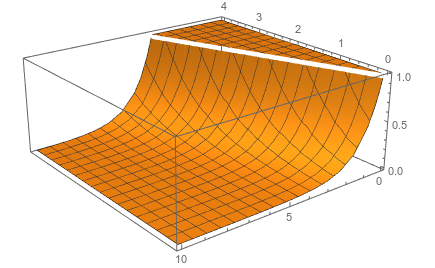
\includegraphics[width=0.75\textwidth]{bvp1}
	\caption{The 3d plot of the solution.}
\end{figure}

The plot in figure \ref{prob1:3d} shows the solution over the 3d field for $0\le x\le10$ and $0 \le \tau \le 4$. The characteristic line can clearly be seen, representing the population count staying constant. This model does not seem realistic because $\lambda$ is 0, meaning that no one dies, the population is essentially immortal and won't stop aging, as can be seen in the 3d plot.


\begin{figure}[H]\label{prob1:3d}
	\centering
	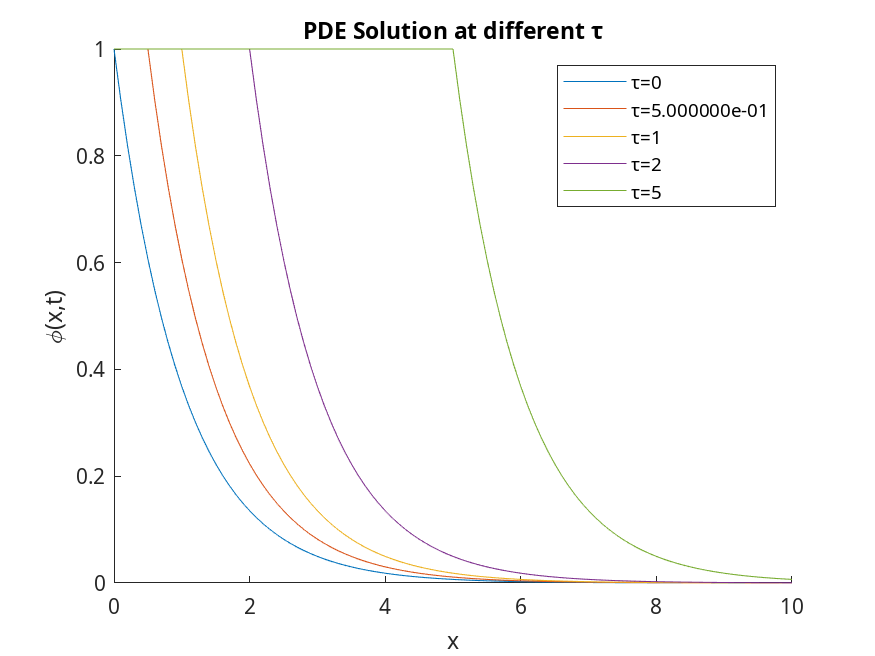
\includegraphics[width=0.75\textwidth]{prob1}
	\caption{The population density at different times.}
\end{figure}
\begin{figure}[H]\label{prob1:3d}
	\centering
	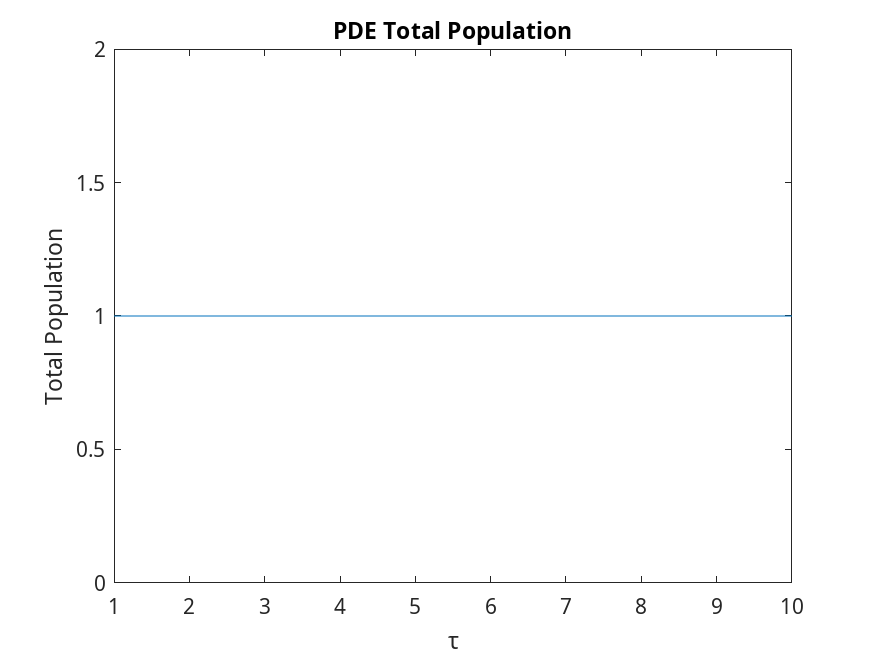
\includegraphics[width=0.75\textwidth]{prob1-pop}
	\caption{The population count over time.}
\end{figure}

\subsection{$\lambda=1$ Constant}
For this inital value problem the value of $\lambda$ is locked at 1. In relation to the model this means that 100\% of people who are born - die. This is a more accurate representation of the real world.
\begin{equation}\label{eq:constant}
	\phi(x, \tau(x)) = F(\tau-x)\cdot\exp(-\lambda(x)\tau(x)) = F(\tau-x)\exp(-\tau)
\end{equation}

The same method used in the previous section is applied to this section to solve the PDE with inital conditions. The first step is to simplify the equation to that seen in figure \ref{eq:constant}. The inital conditions are shown in \ref{eq:iv1} and \ref{eq:iv2}

\begin{equation}\label{eq:iv1}
	\phi(x,0) = \exp(-x) \qquad x \ge 0
\end{equation}

\begin{equation}\label{eq:iv2}
	\phi(0,\tau) = 1 \qquad \tau > 0
\end{equation}

Putting the first initial condition yields the function $\phi(x,\tau) = \exp(-x)$. Again by using a mock variable $\eta$ the inital condition can be used to find the general solution satisfying the initial condition, this can be seen in \ref{eta1}. 

	\begin{align}
		\phi(x,0) = \exp(-x) = F(0-x)\exp(0) \\
		~
		F(-x) = \exp(-x) \qquad F(\eta) = \exp(\eta) \qquad \eta = -x \qquad x \ge 0 \qquad \eta \le 0 \\
		~
		\eta = \tau-x \le 0 \qquad \tau \le x \label{eta1}\\
		~
		\phi(x,\tau) = \exp(\tau-x)\exp(-\tau) = \exp(-x) \qquad \tau \le x
	\end{align}

The second piecewise function can be found by applying the same method to the other inital condition.

	\begin{align}
		\phi(0,\tau) = 1 = F(\tau)\exp(-\tau) \\
		~
		F(\tau) = \exp(\tau) \qquad x \ge 0 \qquad \eta \le 0 \\
		~
		\eta = \tau-x \le 0 \qquad \tau \le x \\
		~
		\phi(x,\tau) = \exp(\tau-x)\exp(-\tau) = \exp(-x) \qquad \tau \le x
	\end{align}

	Since both conditions equal the same function the value of $\phi$ is not piecewise, and is given in whole below.

\[
	\phi(x,\tau) = \begin{cases} 
		\exp(-x) 	& \tau > 0 \qquad x \ge 0
   \end{cases}
\]

The 3d plot can be seen in figure \ref{prob2:3d}

\begin{figure}[H]\label{prob2:3d}
	\centering
	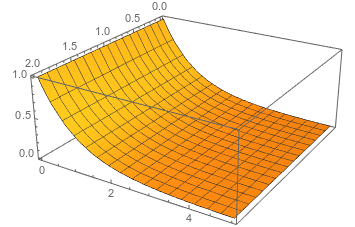
\includegraphics[width=0.75\textwidth]{bvp2}
	\caption{The 3d plot of the solution.}
\end{figure}

The plot in figure \ref{prob2:tau} shows a problem with this model. Because the birth rate is stable the total population does not increase or decrease, it also doesn't change with time. This is not very realistic as most populations vary with time based on enviromental factors.

\begin{figure}[H]\label{prob2:tau}
	\centering
	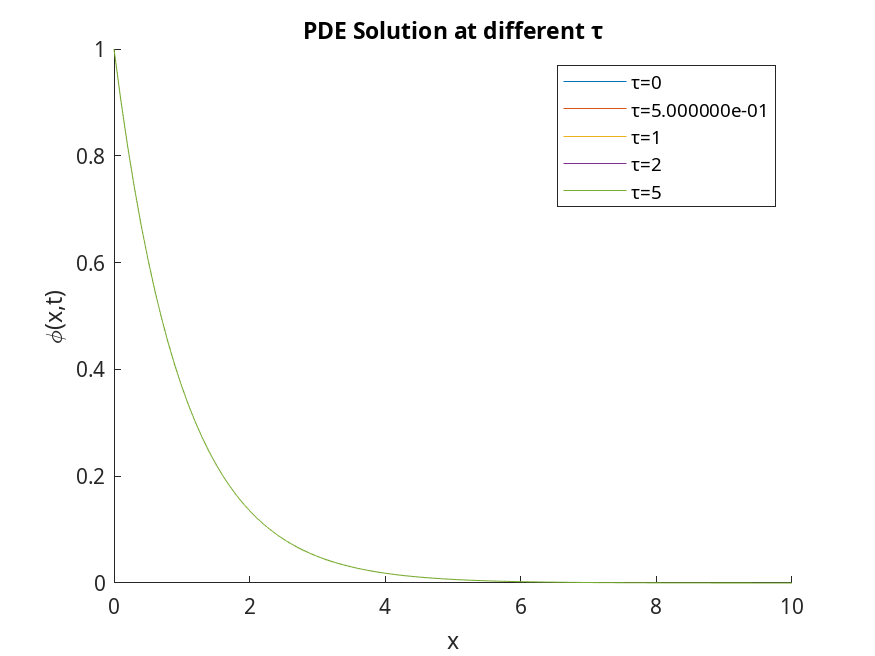
\includegraphics[width=0.75\textwidth]{prob2}
	\caption{The population density at different $\tau$.}
\end{figure}
\begin{figure}[H]\label{prob2:pop}
	\centering
	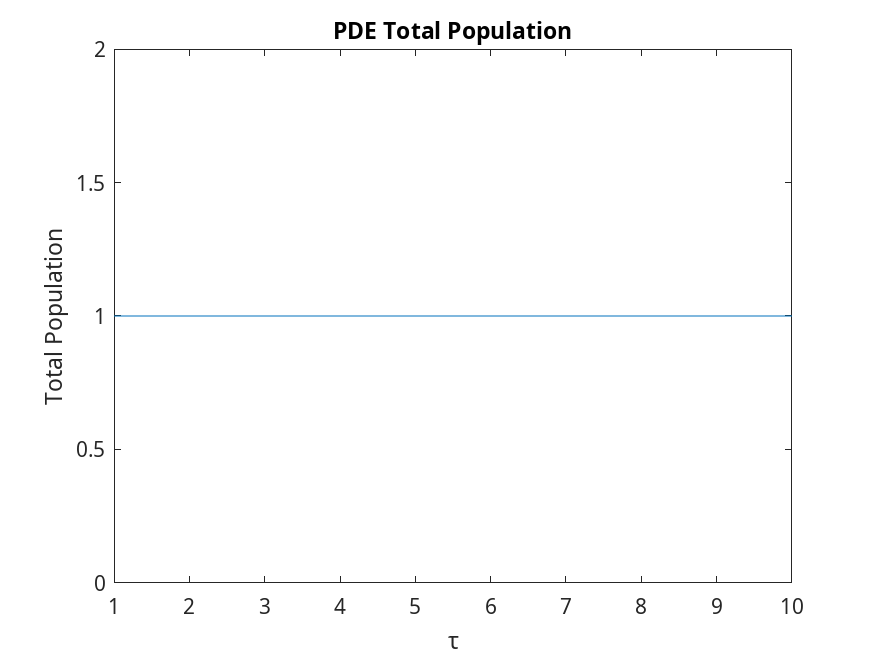
\includegraphics[width=0.75\textwidth]{prob2-pop}
	\caption{The population count over $\tau$.}
\end{figure}

\subsection{Increasing Birthrate}
This IVP describes a population with an inital population density of 0 that has an increasing birth rate defined by $1-\exp(-\tau)$. As before this problem can be solved using the same subsitution and mock value method as before. Starting with the general solution in \ref{eq:gensol} and the intial values defined in \ref{eq:ivp3} an expression for the population density can be found.

\begin{equation} \label{eq:gensol}
	\phi(x, \tau(x)) = F(\tau-x)\cdot\exp(-\tau(x))
\end{equation}

\begin{equation} \label{eq:ivp3}
	\phi(x,0) = 0 \qquad x \le 0, \qquad \phi(0,\tau)=1-\exp(-\tau) \qquad \tau > 0
\end{equation}

Firstly by susituting the first inital condition into our solution the result evaluates to \ref{eq:ivp4}
\begin{align} \label{eq:ivp4}
	\phi(x,\tau) = F(\tau-x)\exp(-\tau) \\
	~
	\phi(x,0) = F(-x)\exp(0) = F(-x) = 0 \\
	\eta = -x \label{mock}\\
	F(\eta) = 0 \qquad \eta \le 0 \\
	F(\tau-x)=0 \label{fn} \qquad \eta=\tau-x \le 0 \qquad \tau \le x\\
	\phi(x,\tau) = 0 \qquad \tau \le x \label{soln:3}
\end{align}

By using a mock variable at \ref{mock} and solving on the characteristic lines where $\eta  =\tau-x$ the solution is shown at \ref{soln:3}. The same method can be done for $\phi(0,\tau)=1-\exp(-\tau)$.

\begin{align}
	\phi(0, \tau) = 1-\exp(-\tau) = F(\tau-x)\exp(-\tau) = F(\tau)\exp(-\tau) \\
	~
	F(\tau) = \exp(\tau)(1-\exp(-\tau)) = \exp(\tau)-1 \\
	\eta = \tau \qquad \eta > 0\\
	F(\eta) = \exp(\eta)-1 \qquad \tau-x = \eta > 0 \qquad \tau > x\\
	F(\tau-x) = \exp(\tau-x)-1 \qquad \tau >x\\
	\phi(x,\tau)=(\exp(\tau-x)-1)\exp(-\tau) = \exp(\tau-x)\exp(-\tau)-\exp(-\tau)\\
	\phi(x,\tau)=\exp(-x)-\exp(-\tau) \qquad \tau >x
\end{align}

Taking the solutions to both piecewise equations gives the final solution below.

\[
	\phi(x,\tau) = \begin{cases} 
		0 						& \tau \le x \\
		\exp(-x)-\exp(-\tau) 	& \tau > x
   \end{cases}
\]

The 3d plot can be seen in figure \ref{prob3:3d}

\begin{figure}[H]\label{prob3:3d}
	\centering
	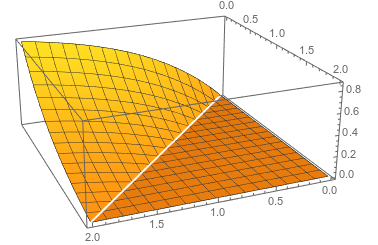
\includegraphics[width=0.75\textwidth]{bvp3}
	\caption{The 3d plot of the solution.}
\end{figure}

\begin{figure}[H]\label{prob2:tau}
	\centering
	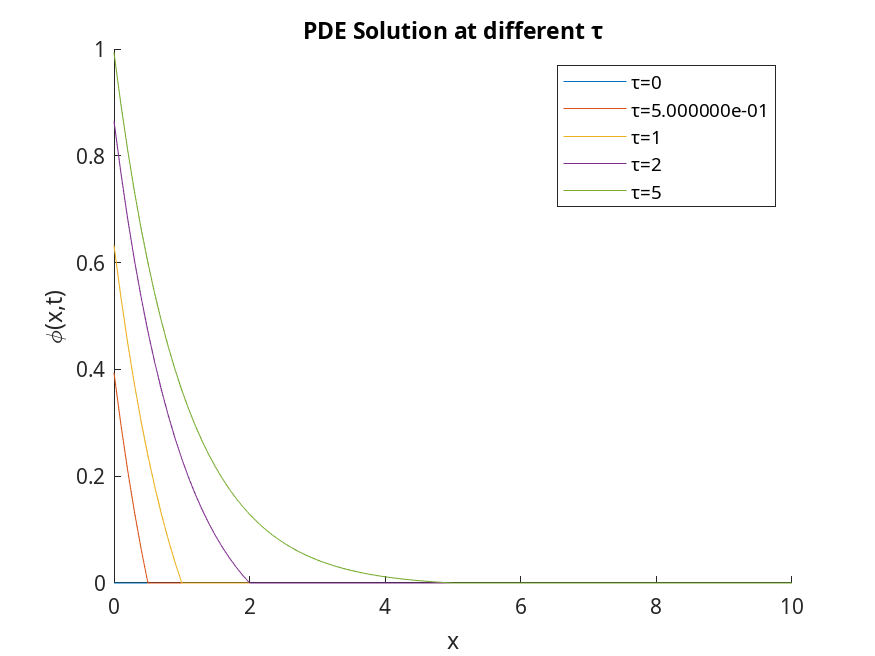
\includegraphics[width=0.75\textwidth]{prob3}
	\caption{The population density at different $\tau$.}
\end{figure}

\begin{figure}[H]\label{prob2:tau}
	\centering
	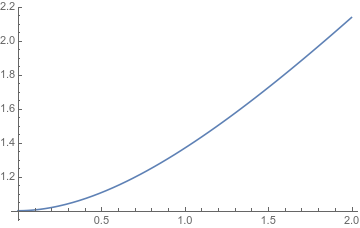
\includegraphics[width=0.75\textwidth]{prob3-pop}
	\caption{The population count at different $\tau$.}
\end{figure}

The model described by these inital and boundary conditons describe a population that starts at 0 and grows proportional to the population. An example of this is an invasive species like rabbits migrating to an area which does not have a rabbit population yet.

\subsection{Decreasing Birthrate}

The final problem relates to a population that has a decreasing birth rate. This is can be modelled with the inital condition of $1-\tau$ between $0 < \tau \le 1$.


\begin{equation} \label{eq:gensol}
	\phi(x, \tau(x)) = F(\tau-x)\cdot\exp(-\tau(x))
\end{equation}

The inital condtions are defined in \ref{initalConditions5}

\begin{equation} \label{initalConditions5}
	\phi(x,0) = \exp(-x) \qquad x \le 0, \qquad \phi(0,\tau)=1-\tau \qquad 0 <\tau \le 1,\qquad \phi(0,\tau)=0 \qquad \tau >1
\end{equation}

Again using the same method of characteristics and mock variables the three pieces of this fucntion can be found. For the first boundary value.

\begin{align}
	\phi(x,0) = \exp(-x) = F(-x) \qquad x \ge 0\\
	~
	\eta = -x \qquad \eta \le 0\\
	~
	F(\eta)=\exp(\eta)\\
	~
	\eta = \tau-x \le 0 \qquad F(\tau-x) = \exp(\tau-x)\\
	~
	\phi(x,\tau) = \exp(\tau-x)\exp(-\tau)=\exp(-x) \qquad \tau \le x
\end{align}

And the second.

\begin{align}
	\phi(0,\tau) = 1-\tau = F(\tau)\exp(-\tau) \qquad 0 < \tau \le 1\\
	~
	F(\tau)=\exp(\tau)(1-\tau) \\
	~
	\eta = -x \qquad \eta \le 0\\
	~
	\eta = \tau \qquad 0 < \eta \le \tau\\
	~
	F(\eta) = \exp(\eta)(1-\eta)\\
	~
	0 <\eta = \tau-x \le 1 \qquad F(\tau-x) = \exp(\tau-x)(1-\tau+x)\\
	~
	\phi(x,\tau) = \exp(\tau-x)\exp(-\tau)(1-\tau+x)=\exp(-x)(1-\tau+x) \qquad 0< \tau-x \le 1
\end{align}

And third.
\begin{align}
	\phi(0,\tau) = 0 = F(\tau) \qquad \tau > 1\\
	~
	\eta = \tau \qquad \eta > 0\\
	~
	F(\eta)= 0 \\
	~
	\eta = \tau-x \qquad \eta = \tau-x>1\\
	~
	F(\tau-x) = 0 \qquad \tau -x >1\\
	~
	\phi(x,\tau) = 0 \qquad \tau-x > 1
\end{align}

Finally combining all three together gives the solutions as per below.

\[
	\phi(x,\tau) = \begin{cases}
		\exp(-x) & \tau \le x\\
		\exp(-x)(1-\tau+x) & 0< \tau-x \le 1 \\
		0 & \tau-x > 1
	\end{cases}
\]
\begin{figure}[H]\label{prob3:3d}
	\centering
	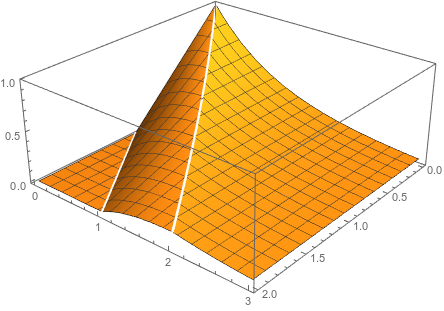
\includegraphics[width=0.75\textwidth]{bvp4}
	\caption{The 3d plot of the solution.}
\end{figure}

\begin{figure}[H]\label{prob2:tau}
	\centering
	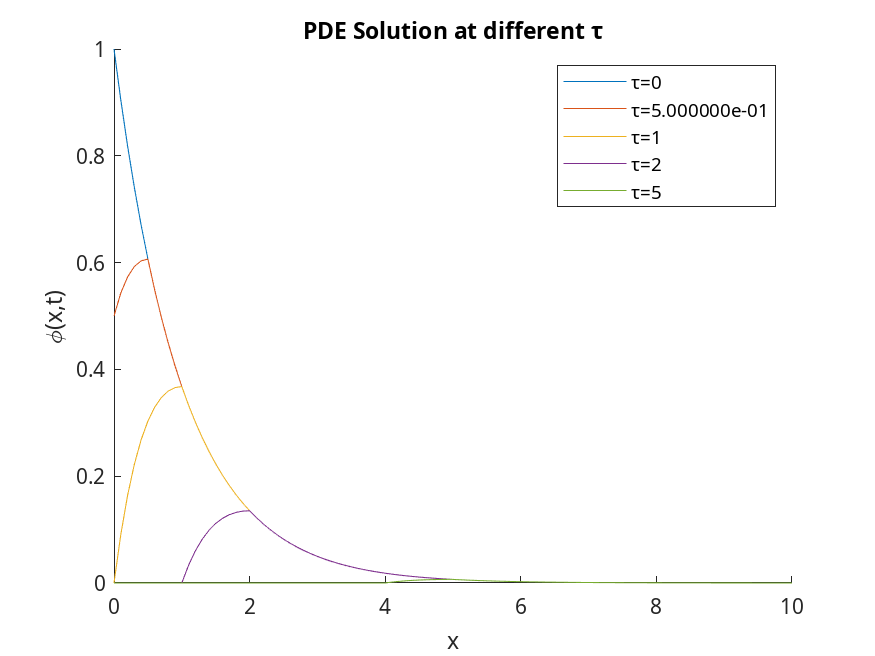
\includegraphics[width=0.75\textwidth]{prob4}
	\caption{The population density at different $\tau$.}
\end{figure}
\begin{figure}[H]\label{prob2:tau}
	\centering
	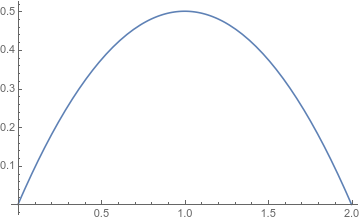
\includegraphics[width=0.75\textwidth]{prob4-pop}
	\caption{The population count at different $\tau$.}
\end{figure}

This solution relates to the second BVP because of it's inital conditions. It's a more realistic scenario because the birth rate is not constant but a function of the population. This can be seen in the 3d plot as the population slowly declines over time.

\end{document}
